\section{Results}
\subsection{The historical coverage gain is reproduced at matched cost}
On the historical six-assay EPA panel, label-0 TAME increased mean minimum-class coverage from 83.739\% to 85.104\%, a gain of 1.3649 percentage points. Operational deferral increased by 2.0164 points, from 42.007\% to 44.023\%, and MacroCSY fell by 1.6067 points, from 48.179\% to 46.572\% (Table \ref{tab:historical}). The expansion recovered some false-active decisions while withholding additional correct positive singletons.

The class-budget-matched omitted-label-probability rule reached the same mean minimum-class coverage, MacroCSY, and deferral. The TAME-minus-probability difference in minimum coverage was 0.0000 points, with a molecule-cluster bootstrap 95\% interval of $[-0.0279,0.0287]$ points. The nondegenerate interval is consistent with differences among individual decisions despite identical aggregate means. This result attributes the historical gain to an attainable error--deferral trade-off rather than additional demonstrated ranking information from transport.

\begin{table}[htbp]\centering\small
\caption{Historical six-assay EPA means with the stack and $\alpha=0.10$. Entries are percentages. The four simple ranking rules use the exact label-0 TAME class budgets. The last row uses the separate active-label objective. $E_0$ is false-active exposure.}\label{tab:historical}
\begin{tabular}{lrrrr}\toprule
Rule & $C_{\min}$ & $E_0$ & MacroCSY & Deferral \\
\midrule
Mondrian LAC baseline & 83.74 & 14.64 & 48.18 & 42.01 \\
TAME, label 0 & 85.10 & 12.93 & 46.57 & 44.02 \\
Omitted-label probability & 85.10 & 12.93 & 46.57 & 44.02 \\
Probability uncertainty & 84.75 & 13.44 & 44.61 & 44.02 \\
Chemical similarity & 84.83 & 13.21 & 45.65 & 44.02 \\
Seeded random selection & 84.87 & 13.24 & 45.34 & 44.02 \\
TAME, label 1 & 83.74 & 14.64 & 48.18 & 42.01 \\
\bottomrule\end{tabular}

\end{table}

The choice of simple comparator was consequential. At the same operational budget, omitted-label ranking obtained 85.10\% minimum-class coverage and 46.57\% MacroCSY, compared with 84.75\% and 44.61\% for probability uncertainty. Similarity and random rankings also gave lower descriptive coverage and yield than omitted-label ranking (Table \ref{tab:historical}). Thus comparison against generic uncertainty alone would overstate the need for transport information. Figure \ref{fig:assays} displays the assay-level results, including the six assays outside the historical panel.

\begin{figure}[htbp]\centering
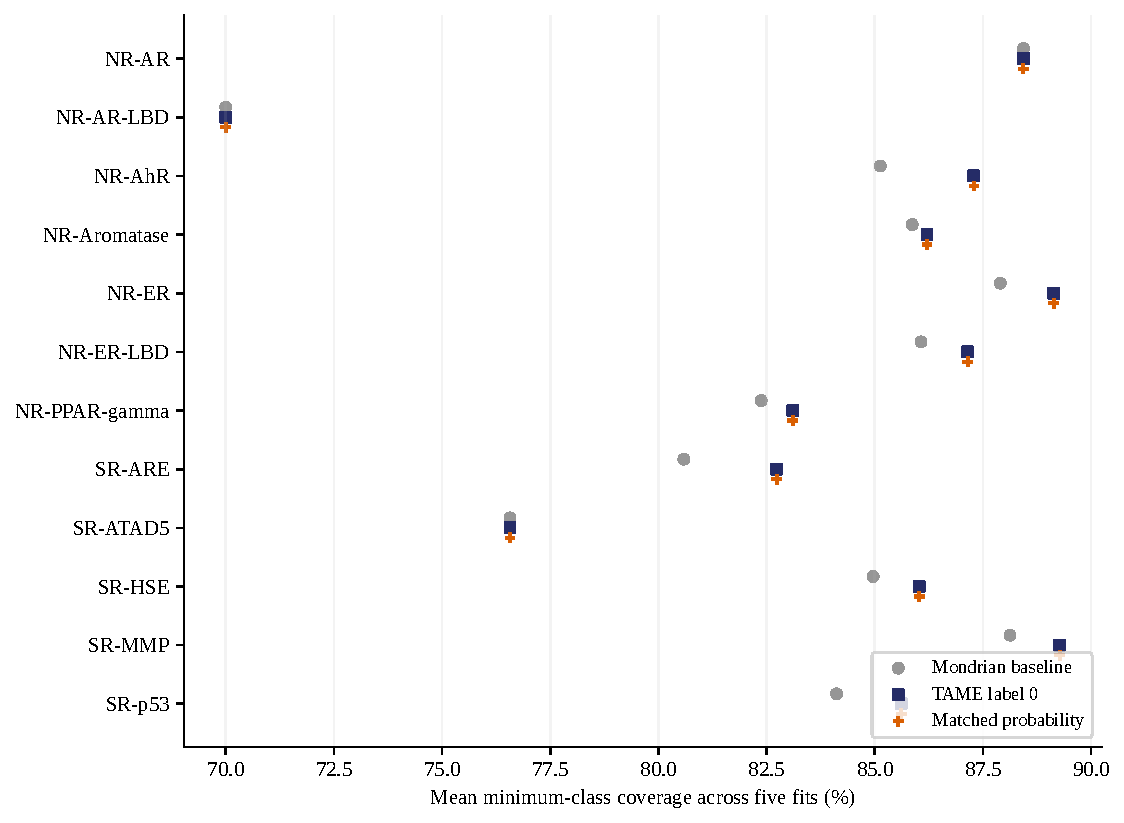
\includegraphics[width=.86\textwidth]{figures/assay_coverage.pdf}
\caption{Assay-level EPA coverage for the stack at $\alpha=0.10$, averaged over five fits. Markers are vertically offset for legibility. Aggregate agreement does not imply identical compound-level selections.}\label{fig:assays}
\end{figure}

\subsection{Gate passage and active-label expansion separate}
In the fixed active-label primary comparison, both transport views passed in every one of the 30 assay--seed cells. Nevertheless, the expansion count was zero in all 30. TAME, its matched comparators, and repaired Mondrian therefore produced the same primary decisions: false-inactive exposure was 10.532\%, minimum-class coverage 83.739\%, and operational deferral 42.007\%. The reported zero difference and degenerate bootstrap interval arise from no intervention in this panel; they do not measure the relative quality of two nonempty rankings.

Across all twelve EPA assays, both views passed in all 180 classical predictor cells. For the stacked predictor, active-label TAME added 21 compound--fit deferrals, concentrated in NR-AR and NR-AR-LBD. Seven were selected only by TAME and seven only by the matched probability rule. Neither rule recovered a false-inactive decision among these additions. Because the sums span fitted repetitions, they count repeated decisions rather than independent compounds (Table \ref{tab:activation}).

\begin{table}[htbp]\centering\small
\caption{Active-label mechanism counts at $\alpha=0.10$ with the stack. Pass requires both views. Added counts are equal for TAME (A) and matched probability (P); A-only/P-only denotes discordant selections. Rescued lists erroneous inactive decisions recovered by A/P. Counts sum over fit seeds; the two EPA rows overlap.}\label{tab:activation}
\begin{tabular}{lrrrr}\toprule
Setting & Pass / cells & Added & A-only / P-only & Rescued \\
\midrule
EPA, historical six & 30 / 30 & 0 & 0 / 0 & 0 / 0 \\
EPA, all twelve & 60 / 60 & 21 & 7 / 7 & 0 / 0 \\
AMES / random & 5 / 5 & 0 & 0 / 0 & 0 / 0 \\
CYP2D6 / random & 5 / 5 & 0 & 0 / 0 & 0 / 0 \\
DILI / random & 0 / 5 & 0 & 0 / 0 & 0 / 0 \\
hERG / random & 0 / 5 & 0 & 0 / 0 & 0 / 0 \\
AMES / scaffold & 5 / 5 & 0 & 0 / 0 & 0 / 0 \\
CYP2D6 / scaffold & 5 / 5 & 19 & 0 / 0 & 1 / 1 \\
DILI / scaffold & 0 / 5 & 0 & 0 / 0 & 0 / 0 \\
hERG / scaffold & 0 / 5 & 0 & 0 / 0 & 0 / 0 \\
\bottomrule\end{tabular}

\end{table}

\subsection{Additional assay families distinguish fallback from nonactivation}
AMES and CYP2D6 passed both transport gates in every shared-predictor fit under both split regimes. hERG failed the 100-calibration-observation threshold. DILI also had fewer than 100 target structures. Their active-label rules consequently retained the baseline. These are different reasons for observing a zero matched effect.

For the stack, all four random-holdout tasks had zero additional deferrals. The scaffold CYP2D6 analysis added 19 compound--fit deferrals, identical under TAME and matched probability; both recovered one false-inactive decision. Its false-inactive exposure decreased from 10.410\% to 10.369\%, with deferral increasing from 34.375\% to 34.520\%. The remaining stacked scaffold tasks added no deferrals.

Across all 24 endpoint/split/predictor active-label comparisons, 23 had zero error differences. The remaining CYP2D6 random-split equal-logit contrast was $-0.0418$ points, with a pointwise interval of $[-0.1330,0.0000]$. The experiment therefore distinguishes small-sample fallback, eligible but inactive expansion, and a small nonempty expansion reproduced by the simple ranking rule.

\subsection{Predictor, workload, and reference-system comparisons}
The underlying predictor changes the trade-off even before transport expansion. On the historical panel, ordinary equal-logit Mondrian had 84.82\% minimum-class coverage and 46.70\% MacroCSY at 44.37\% deferral; logistic Mondrian had 84.84\%, 43.51\%, and 47.58\%, respectively. The stack had lower minimum coverage but higher MacroCSY and fewer deferrals (Supplementary Table S3). Comparing one column could conceal these differences.

The fixed-workload curves show how coverage can rise as additional decisions are withheld (Figure \ref{fig:workload}). At its native operating point, deterministic Mondrian APS reached 91.38\% minimum-class coverage and zero false-inactive exposure, while deferring 89.68\% of eligible targets and retaining 9.28\% MacroCSY. Its apparent coverage advantage is accompanied by a large reduction in informative decisions.

The neural reference systems likewise occupied different operating points. The swapped-margin CoDrug candidate-class variant gave 10.93\% false-inactive exposure at 36.58\% deferral and 52.97\% MacroCSY. Selective KMM with candidate-label thresholds gave 7.67\% false-inactive exposure at 52.79\% deferral and 36.27\% MacroCSY. All ten declared reference configurations, including the printed-margin CoDrug and predicted-group KMM interpretations, appear in Supplementary Table S4. These complete-system comparisons describe the trade-offs of different predictors and uncertainty rules.

\begin{figure}[htbp]\centering
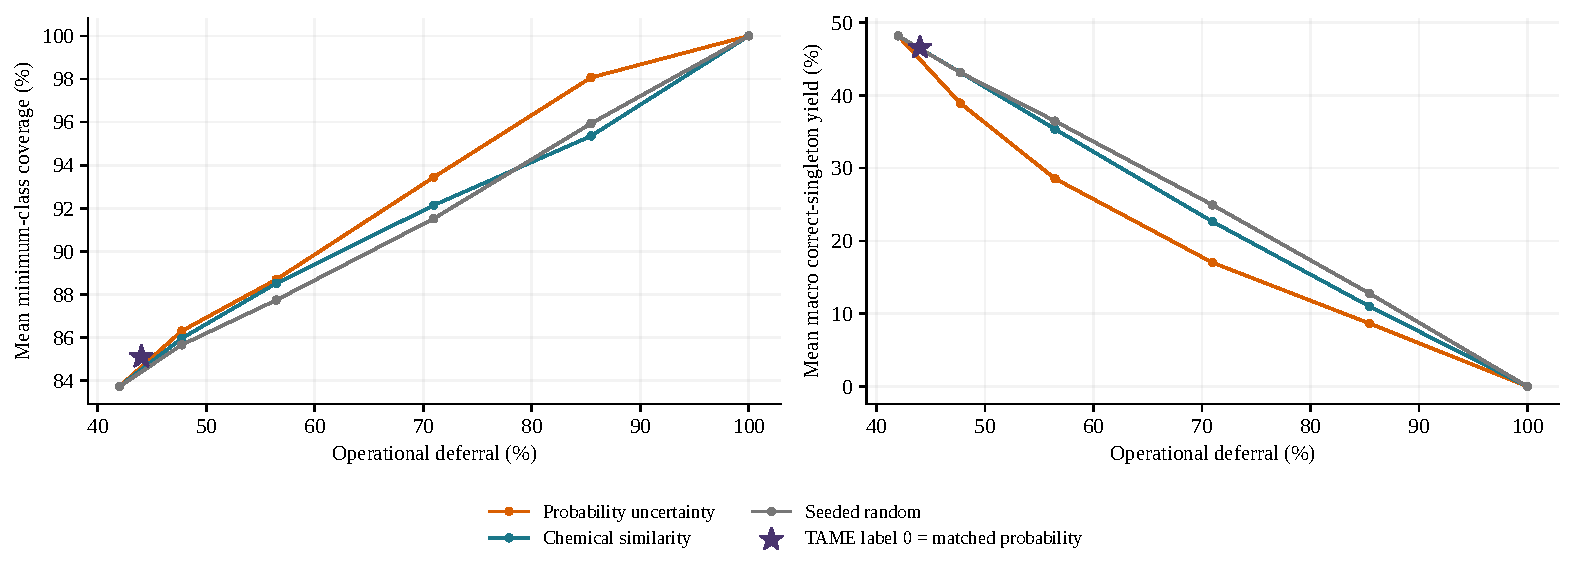
\includegraphics[width=\textwidth]{figures/workload_tradeoff.pdf}
\caption{Coverage and correct-singleton yield across fixed additional-deferral fractions on the historical EPA panel. The star marks the label-0 TAME and matched-probability point. They share these aggregate coordinates. Curves use uncertainty, similarity, or random ranking over the baseline singleton pool; they describe workload trade-offs rather than class-budget-matched effects at every point.}\label{fig:workload}
\end{figure}

\subsection{Ablations localize the absence of added targeting information}
Removing gates did not activate the stack's primary active-label expansion. A physicochemical-only view or view union added sixteen decisions in one primary assay--seed cell; their own-budget error difference was $-0.0952$ points, with an interval of $[-0.3030,0.0000]$. Across 280 declared own-budget ablation and query-alignment contrasts, no pointwise error interval excluded zero. The five gated and five ungated query-weight permutations each produced zero primary-panel budget, making that panel uninformative about the value of query-specific alignment.

In the synthetic paired no-shift and changed-conditional scenarios, all thirty pairs shared identical prediction and transport-diagnostic inputs. Active-label TAME nevertheless had mean class-1 coverage of 90.36\% and 39.74\%, respectively, with the same 30.30\% deferral. This mechanism check illustrates why diagnostics based only on the observed covariates cannot identify a changed conditional outcome law.

\section{Discussion}
The main empirical finding is that the historical coverage improvement survives recomputation but loses its interpretation as extra transport-based error targeting. An omitted-label-probability rule reproduces the 1.3649-point minimum-coverage gain at the same predicted-class budget. The framework makes this distinction measurable without changing the predictor or using target outcomes to rank compounds. It also shows why the strongest relevant simple comparator depends on the decision being deferred: a rule tailored to the omitted label can outperform generic probability uncertainty at identical cost.

The activation condition explains a second issue that aggregate accuracy tables obscure. A view can satisfy every diagnostic gate and still fail to add the protected label to any baseline singleton. In that case, zero matched differences reflect an unused intervention. Conversely, an expansion can occur without rescuing an error, as in the all-twelve-assay active-label result. Reporting gate eligibility, additions, discordant selections, and recovered errors in sequence connects the mathematical rule to the actual decisions.

The constant-query-weight result clarifies what transport weighting can contribute. With fixed query mass, changing source weights or a cell-level gate can move the probability threshold and hence the budget, but cannot change the within-pool ordering. Query-dependent thresholds can depart from that ordering; useful departures must concentrate errors more effectively at equal cost. The molecular results offer a direct test of this distinction, while leaving room for other predictors, shifts, and density estimators to produce different outcomes.

The scope of the evidence is a fixed collection of assays and molecular cohorts. Repeated fits quantify model variation but reuse compounds; the shared-structure bootstrap preserves this dependence. The additional families supply random/scaffold holdout checks, with visible small-sample fallback in hERG and DILI. Estimated and clipped ratios also differ from known likelihood ratios under exact covariate shift. These distinctions define what the reported comparisons estimate.

For molecular screening, the useful output is a joint account of recovered errors, surrendered correct decisions, and operational workload. A coverage gain can be scientifically informative even when a complex rule does not win: here it identifies a reproducible, simpler route to the same observed trade-off and provides an explicit test for when a transport-based expansion contributes information beyond that route.

\section{Conclusion}
Class-budget matching and an exact activation condition separate the cost and targeting components of molecular prediction-set expansion. In the evaluated TAME study, a simple omitted-label-probability ranking reproduced the historical coverage gain, while the prespecified active-label expansion was inactive on the primary panel. Reporting eligibility, intervention, and error recovery together gives a more informative assessment of molecular uncertainty procedures than coverage alone.

\section*{Data and code availability}
The data adapters, experiment suite, frozen aggregate inputs, manuscript sources, and rebuilding scripts are available in the \href{https://github.com/DCarchimonde/aidd-paper-factory/tree/paper2-tame-resubmission-20261112/paper2_latex/resubmission_20261112}{versioned project directory}. The complete numerical supplement retains all returned cell metrics, panel metrics, and paired contrasts. The manuscript rebuilding script operates on frozen aggregates; retraining and molecule-level inference use the experiment suite and its full exports.
\section*{Declaration of competing interest}
The authors declare no competing interests.
\section*{Funding}
The authors received no specific funding for this work.
\section*{CRediT authorship contribution statement}
Siyuan Tong: Conceptualization, Methodology, Software, Validation, Formal analysis, Investigation, Data curation, Visualization, Writing -- original draft, Writing -- review \& editing. Yuechen Wang: Methodology, Validation, Writing -- review \& editing.
\section*{Declaration of generative AI and AI-assisted technologies}
OpenAI ChatGPT was used for language editing, manuscript organization, LaTeX formatting, code assistance, and preparation of reproducibility materials. The authors are responsible for the content of the submitted manuscript.
